\section{Annexes}

\subsection{Decomposition by continuous change}

The model of continuous change \citep{horiuchiDecompositionMethodBased2008} is used to decompose the change in aggregate labour supply between 2005 and 2025 (the dependent summary measure) into additive effects associated with changes in demographic and behavioural components (the covariates). The model decomposes the difference between two summary measures generated by the same process into several components, each representing the contribution of an underlying factor. The process is defined as a function \(f\), which takes the values of the factors as arguments and returns a summary measure.

\vspace{0.7em}\par
\citet{horiuchiDecompositionMethodBased2008} demonstrates that as the factors transition from values \(x_i(t_1)\) to \(x_i(t_2)\) between two times \(t_1\) and \(t_2\), the summary measure changes from \(f(x_i(t_1))\) to \(f(x_i(t_2))\), and the difference between these two measures can be decomposed into additive components \(c_{i}\) representing the contribution of changes within each factor to this difference. This is expressed by equation \eqref{eq:hofr}.

\begin{equation} \label{eq:hofr}
    f(x_i(t_2)) - f(x_i(t_1)) = \displaystyle\sum_{i}c_{i}
\end{equation}

\vspace{0.7em}\par
With \(i = 1, 2, ..., n\) being the factors involved. The decomposition is based on the assumption that the change in the covariate \(x_i\) occurs continuously or gradually over a real or hypothetical time dimension \(t_1 \rightarrow t_2\). This provides a reasonable justification for the additivity of the effects of the factors and the elimination of interaction terms even if the process in question is a non-additive function of the covariates \citep[p.~786]{horiuchiDecompositionMethodBased2008}.

\vspace{0.7em}\par
In other words, the continuous change model (CCM) introduces a decomposition function \(g\) which, using a process function \(f\), transforms two series of covariates, the vectors \(X(t_1)\) and \(X(t_2)\) representing the values of the covariates \(X = (x_1, ..., x_i, ..., x_n)\) at times \(t_1\) and \(t_2\), into a series of contributions or effects, the vector \(C = (c_1, ..., c_i, ..., c_n)\). Thus, we can write:

\begin{equation}\label{eq:gfr}
    C = g(X, f)
\end{equation}

The series \(X\) and \(C\) having the same lengths, results in a perfect correspondence between the factors and the effects, which can be grouped for analysis purposes. Furthermore, the idea of continuity implies that each element \(c_i\) of the series \(C\) is obtained by integration according to the equation:

\begin{equation}\label{eq:mxfr}
    c_i = \int_{x_i(t_1)}^{x_i(t_2)} \frac{\partial f(t)}{\partial x_i(t)} dx_i(t)
\end{equation}

In practice, equation \eqref{eq:mxfr} is estimated by numerical integration where \(\int_{x_i(t_1)}^{x_i(t_2)} d(t)\) is approximated by \(\sum_{x_i(t_1)}^{x_i(t_2)} \delta(t)\), with \(x_{it} = x_i(t)\) being the value of a factor \(i\) at a moment \(t\). Adapting the continuous change model to measure equation \eqref{eq:pclab} allowed the total variation in the aggregate labor supply between 1981 and 2016 to be distributed not only among these three components but also by age group and residence status (immigrants and natives). For this article, the decomposition was performed by creating an auxiliary function \(g\) around the R package \citep{Rstat:2018} DemoDecomp \citep{DemoDecomp:2018}. The code and data used are available upon request.

\vspace{0.7em}\par
The CCM model is a better alternative to the standardization method often used in demography to account for differences in population structure when comparing demographic measures. Indeed, standardization requires a third population to serve as a standard, making it somewhat less robust as different standards can lead to different results. The CCM model solves this problem and allows for direct decomposition without interaction terms between the different factors.

Interaction effects in regression analysis refer to situations where the impact of one variable on a dependent variable is not constant or additive but depends on the values of other variables. In traditional decomposition methods, such as standardization, any discrepancy between the overall change and the sum of the individual effects of the variables is also called an interaction effect. In such cases, the interaction represents an incomplete separation of the contributions of individual covariates to the overall change or difference in a dependent variable.


\subsection*{Data Source and Variables}

The analysis uses microdata from the \textit{Encuesta de Población Activa} (EPA), Spain's quarterly Labour Force Survey produced by the National Statistics Institute (INE). The EPA is a nationally representative household survey covering the population aged 16 and over. It follows a stratified, two-stage sampling design, with census sections as primary sampling units and dwellings as secondary units. Each quarterly wave includes approximately 46{,}000 dwellings and more than 100{,}000 individuals. INE provides calibrated survey weights to ensure consistency with population totals by sex, age, and region. The microdata contain detailed demographic characteristics, labour-force status, employment conditions, hours worked, and place of birth. The original variables used from the microdata files are:

\begin{itemize}
    \item \textbf{FACTOREL (survey weight)}: Expansion factor assigned to each respondent, derived from the sampling design and calibrated to external population benchmarks. It is used to compute weighted totals and representative aggregates.

    \item \textbf{EDAD1 / EDAD5 (age group)}: Age information is provided in grouped intervals. Across releases, the relevant age-group variable appears as either \textit{EDAD1} or \textit{EDAD5}, but both use five-year age groups for the analytical period. The analysis uses whichever variable is available and standardises it into a single age-group variable.

    \item \textbf{AOI (labour-force status)}: Constructed by INE from responses on work activity, job search, and availability. \textit{AOI} classifies individuals as employed, unemployed, or inactive. It is used to identify employed persons and the active population.

    \item \textbf{HORASH (effective weekly hours worked)}: For employed respondents, the EPA records actual hours worked in the reference week, including overtime and excluding absences. These responses are coded into \textit{HORASH} and used to compute average hours and total hours supplied.

    \item \textbf{PRONA1 (province or country of birth)}: Respondents report their place of birth, which INE codes as Spanish provinces or foreign countries. This variable is used to distinguish Spanish-born from foreign-born individuals.
\end{itemize}


\subsection{Trend in labour force components}

\begin{figure}[H]%
    \caption{Average participation rate by major age groups for immigrants and natives, Spain 2005-2025}
    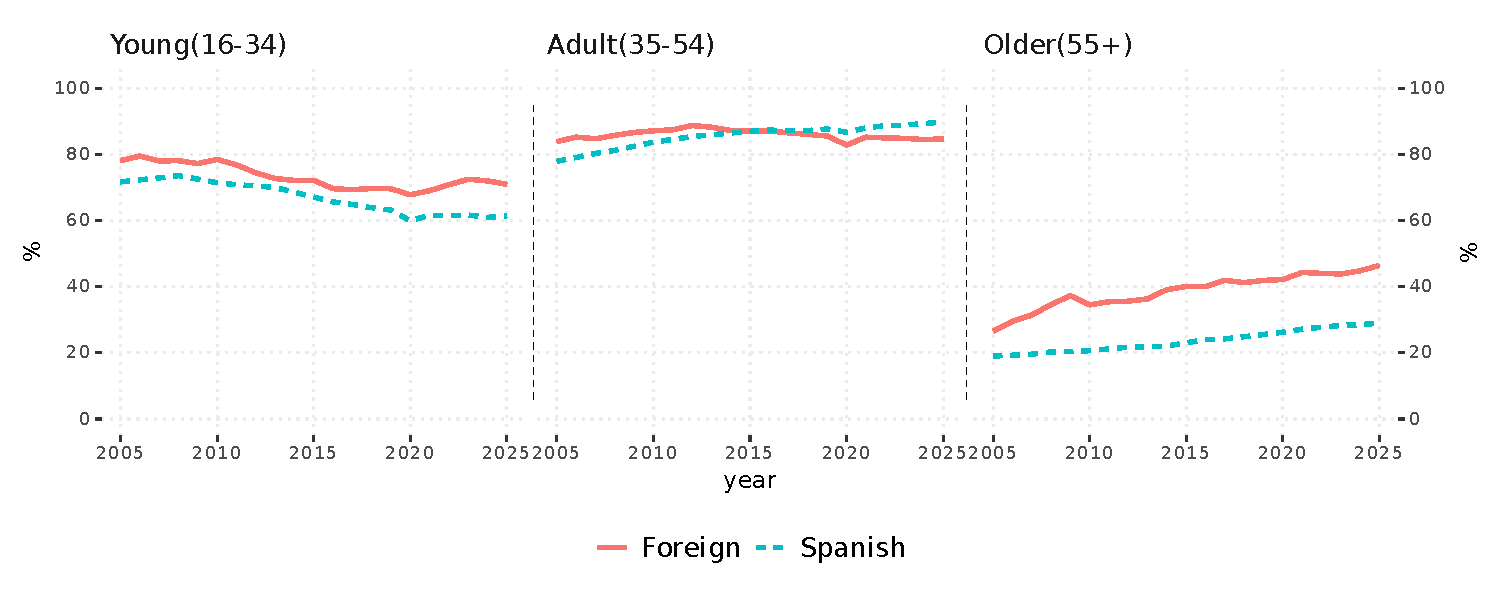
\includegraphics[width=1\textwidth]{../resrc/wpx.pdf}%
    \label{fig:wpx}%
\end{figure}%

\begin{figure}[H]%
    \caption{Average worked hours by major age groups for immigrants and natives, Spain 2005-2025}
    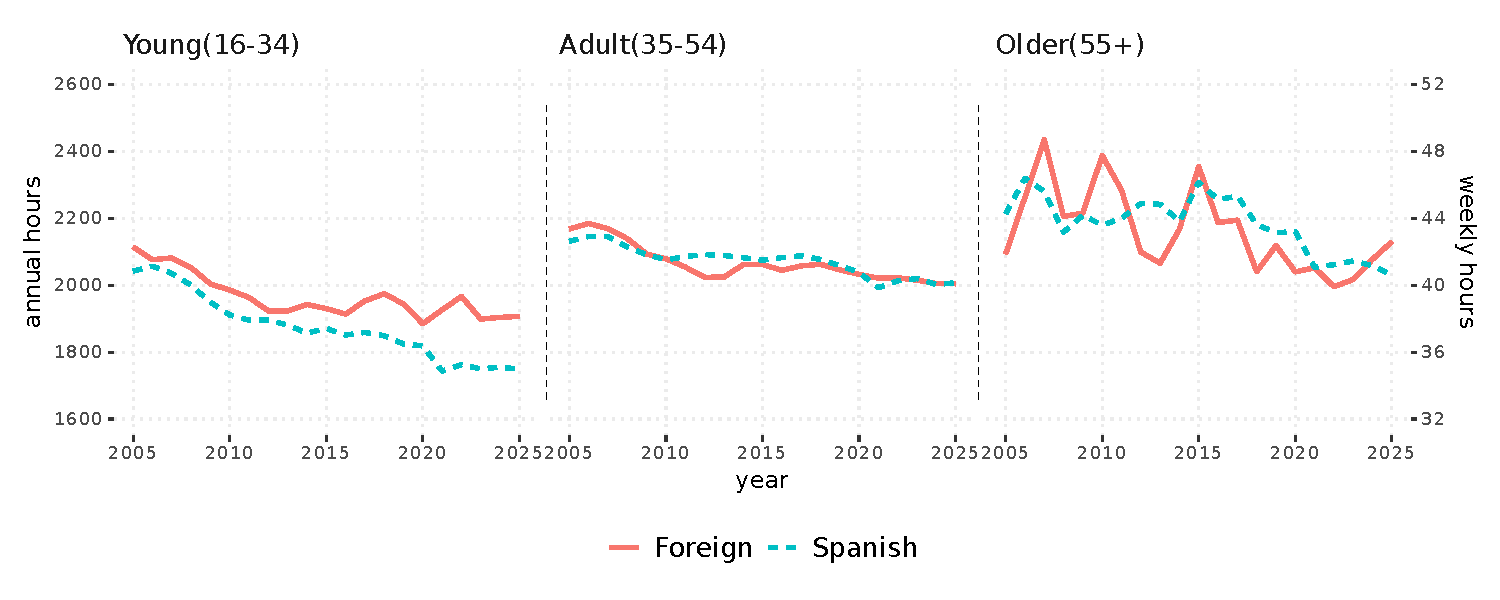
\includegraphics[width=1\textwidth]{../resrc/whx.pdf}%
    \label{fig:whx}%
\end{figure}%

\begin{figure}[H]%
    \caption{Percentage of total population by major age groups for immigrants and natives, Spain 2005-2025}
    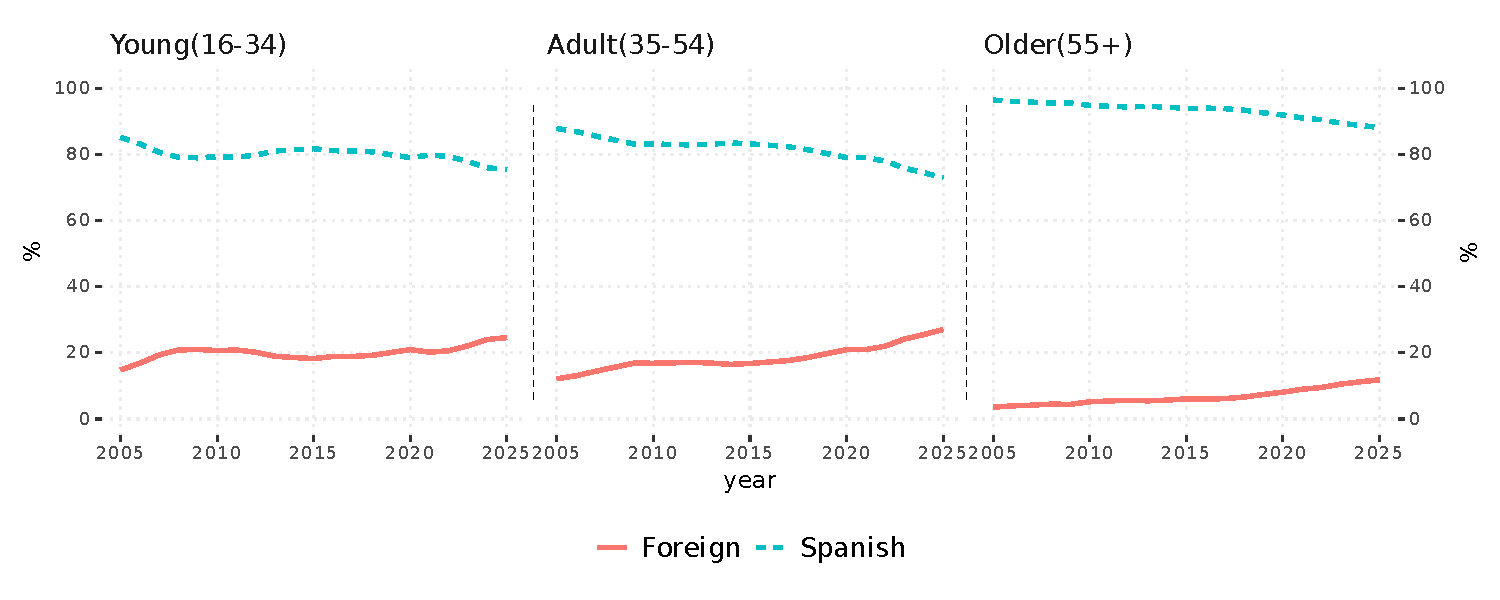
\includegraphics[width=1\textwidth]{../resrc/stx.pdf}%
    \label{fig:stx}%
\end{figure}%

\begin{figure}[H]%
    \caption{Total population aged 16+ in full-time equivalent (FTE) by birthplace, Spain 2005-2025}
    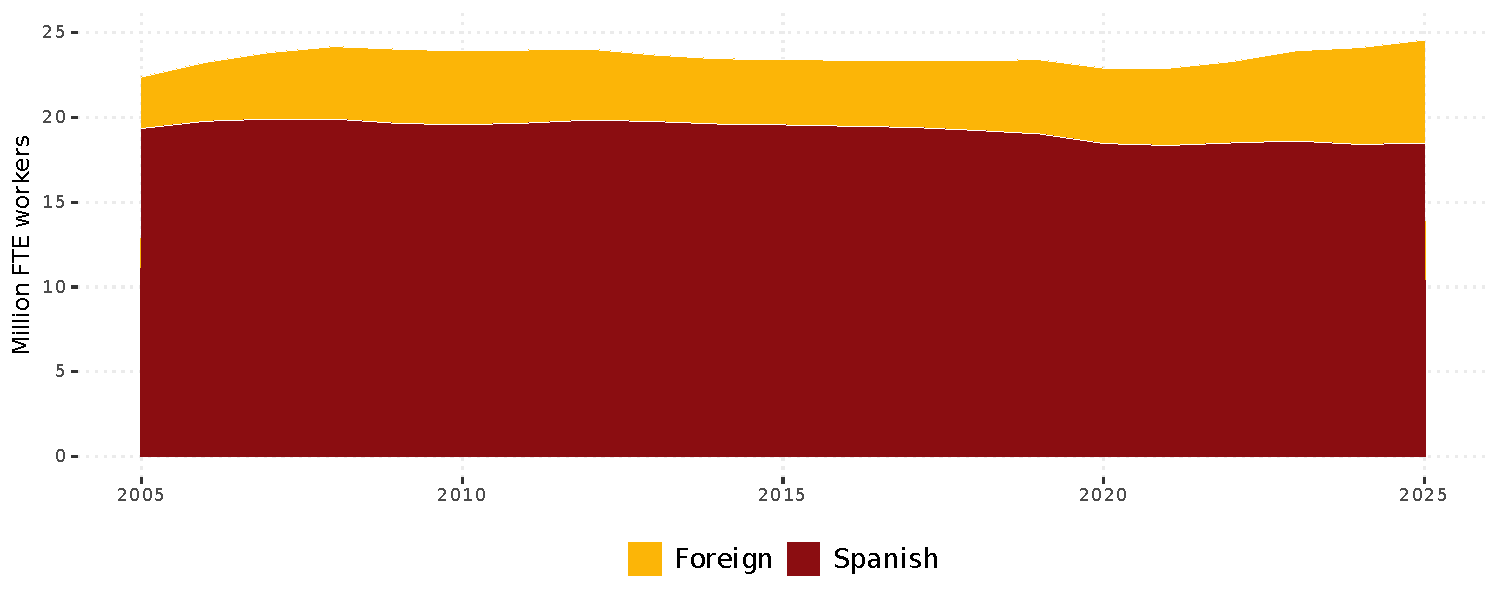
\includegraphics[width=1\textwidth]{../resrc/labchg.pdf}%
    \label{fig:labchg}%
\end{figure}%
